  %%%%%%%%%%%%%%%%%%%%%%%%%%%%%%%%%%%%%%% -*- coding: utf-8; mode: latex -*- %%
  %
%%%%%                         CHAPTER
 %%%
  %

% $Id: 1020-lorem-ipsum.tex,v 1.2 2009/06/19 15:51:46 david Exp $
% $Log: 1020-lorem-ipsum.tex,v $
% Revision 1.2  2009/06/19 15:51:46  david
% *** empty log message ***
%
% Revision 1.1  2007/11/23 09:52:39  david
% *** empty log message ***
%
%

  %%%%%%%%%%%%%%%%%%%%%%%%%%%%%%%%%%%%%%%%%%%%%%%%%%%%%%%%%%%%%%%%%%%%%%%%%%%%%
  %
%%%%%                           HEAD MATTER
 %%%
  %

\chapter{Read-Only Root Level Single Snapshot Implementation and Evaluation}
%\addcontentsline{lof}{chapter}{\thechapter\quad Lorem Ipsum}
%\addcontentsline{lot}{chapter}{\thechapter\quad Lorem Ipsum}
\label{ch:RONSIE}



  %%%%%%%%%%%%%%%%%%%%%%%%%%%%%%%%%%%%%%%%%%%%%%%%%%%%%%%%%%%%%%%%%%%%%%%%%%%%%
  %
%%%%%                        FIRST SECTION
 %%%
  %

\section{Evaluation}
\textbf{Cluster Configuration}\\
MySql Cluster with 6 data nodes and 1 management server is used for evaluation.The management server which also host mysql server deamon.\\
Management Server\& Data Nodes: 40GB RAM, 24 Intel(R) Xeon(R) CPU X5660  @ 2.80GHz each with 6 Cores.\\

The roll back algorithm mentioned in \ref{alg:ROSSRB} is implemented using a thread pool, where each thread processes given number of table records [100,000]. The implementation is executed at MySql server as well as via directly connecting NDB-Cluster\cite{29} with ClusterJ\cite{clusterj}. 

The results with evaluation at MySql Server are shown below.\\
\begin{center}
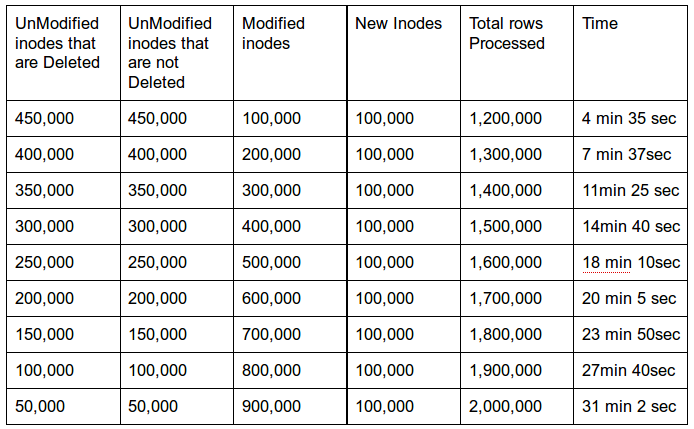
\includegraphics[scale=0.65]{figs/preliminar/MySqlServerSingleSnapshotEval.png}
\captionof{figure}{Benchmark on MySqlServer}\label{fig:MySqlServerSSE}%
\end{center}

\pagebreak

\begin{center}
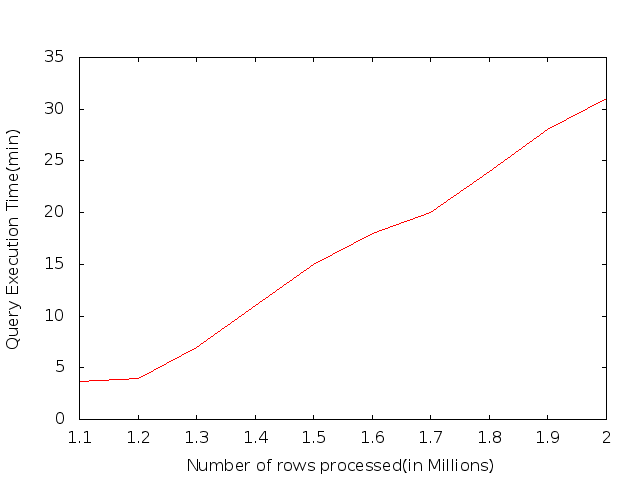
\includegraphics[scale=0.65]{figs/preliminar/MySqlServerSingleSnapshotEvalGraph.png}
\captionof{figure}{Benchmark-Graph on MySqlServer}\label{fig:MySqlServerSSEGraph}%
\end{center}

The high execution time with MySql server is because of update of column which is a primary key, in this case id,which we are changing from its negative value to positive value. In evaluations with clusterJ, batch size of rows were read, for each row a new row with id negative of the former row's id is inserted. 

%The results with evaluation by ClusterJ  are shown below.\\
%\begin{center}
%\includegraphics[scale=0.65]{figs/preliminar/ClusterJSingleSnapshotEval.png}
%\captionof{figure}{Benchmark on ClusterJ}\label{fig:ClusterJSSE}%
%\end{center}

\pagebreak

%\begin{center}
%\includegraphics[scale=0.65]{figs/preliminar/ClusterJSingleSnapshotEvalGraph.png}
%\captionof{figure}{Benchmark-Graph on ClusterJ}\label{fig:ClusterJSSEGraph}%
%s\end{center}




  %%%%%%%%%%%%%%%%%%%%%%%%%%%%%%%%%%%%%%%%%%%%%%%%%%%%%%%%%%%%%%%%%%%%%%%%%%%%%
  %
%%%%%                         ANOTHER SECTION
 %%%
  %


  %
 %%%
%%%%%                        THE END
  %
  %%%%%%%%%%%%%%%%%%%%%%%%%%%%%%%%%%%%%%%%%%%%%%%%%%%%%%%%%%%%%%%%%%%%%%%%%%%%%

%%% Local Variables: 
%%% mode: latex
%%% TeX-master: "tese"
%%% End: 
